\documentclass[twocolumn]{preport}
\usepackage[dvipdfmx]{graphicx}
\graphicspath{{figs/}}

\title{2017年中間試問要旨:\\
等身大ヒューマノイドにおける実環境での状況認識と動作学習に関する研究}
\author{稲葉・岡田研究室  指導教員 稲葉雅幸 教授\\
  機械情報工学科4年 03-160274 大森 悠貴 }

\begin{document}

\pagestyle{empty}
\maketitle
\thispagestyle{empty}
\sloppy

\section{はじめに}
日常生活環境、特に室外環境で人間とロボットが共に過ごすためには、認識や行動の高速化が求められる。
これらの素早い認識、行動が特に求められるのは主に動的環境下においてである。
しかし、動的な環境で正確な認識が難しい、またシミュレータ上で完全なモデルが作成できないことから、ダイナミックな動きをするとシミュレータと実際の環境での差異が生じてしまう。
そのため、実際の環境の不確実な情報からでも、ある程度適切な動作生成ができるようになることが必要である。

高速な動作生成をしている先行研究として、石川ら\cite{Ishikawa}の高速バッティングの研究があるが、カメラとロボットが分離しおり、スタンドアローンでの行動実現を目指すためにはカメラをロボットに搭載する必要があり、この手法はそのまま適応できない。また寺澤ら\cite{Terasawa}の高速スイングはオフラインで軌道を生成してその動きを再生しており、認識に基づいた動作生成ができていない。

本研究では、素早い認識と動作生成が求められる行動として、テニスのボレー動作を題材に選んだ。このような動作を実現するため、比較的速い動作が可能なヒューマノイドロボットであるJAXON2\cite{Kojima}を用いて研究を行う。


%% 将来的にヒューマノイドロボットが日常生活環境で動作する際、すぐにその環境に馴染んで本来持つパフォーマンスができることが望ましい。特定の環境下でしか動作できないのは望ましくない。
%% 現状、ある環境にロボットを適応させるには、その環境でのチューニングをしなければならないことが多い。
%% また日常生活環境は常に変化する環境である。こうした外界の状況を把握するためにも


%% 本稿はプログレスレポートのテンプレートである\cite{Sakai}.

%% 本稿における「、」や「。」は、\verb|make pub|を実行することで、「,」や「.」に変更される。

%% 図は\figref{nowprinting}や\tabref{sample}として参照する.

%% \begin{figure}[tbh]
%%  \begin{center}
%%   \begin{minipage}{0.3\columnwidth}
%%    \includegraphics[width=\columnwidth]{nowprinting.eps}
%%    \caption{eps図の参考例}
%%   \end{minipage}
%%   \hspace{0.15\columnwidth}
%%   \begin{minipage}{0.3\columnwidth}
%%    \includegraphics[width=\columnwidth]{dj.jpg}
%%    \caption{jpg図の参考例}
%%   \end{minipage}
%%   \label{figure:nowprinting}
%%  \end{center}
%% \end{figure}

\section{ボレー動作実現へのアプローチ}
%% ボールの軌道予測をする場合、環境中にカメラを複数台セットして軌道を予測するものもあるが、本研究では環境に依存しない動作生成を目指すため、ロボット自身にカメラを取り付けている
%% ロボットによるバッティングでは高速カメラを使うアプローチ\cite{Ishikawa}と予測を用いるアプローチがあるが、ヒューマノイドの動作生成には時間が一定以上かかるという観点から、後者のアプローチを用いる
%% 三次元座標の計算はそれぞれの二次元座標上のボールの重心から計算している
不確実な情報から
\figref{system}
入力を

\begin{figure}[tbh]
 \begin{center}
  \begin{minipage}{0.65\columnwidth}
   \includegraphics[width=\columnwidth]{coordinates_graph_316.png}
   \caption{システム構成図}
   \label{figure:system}
  \end{minipage}
  \hspace{0.02\columnwidth}
  \begin{minipage}{0.3\columnwidth}
   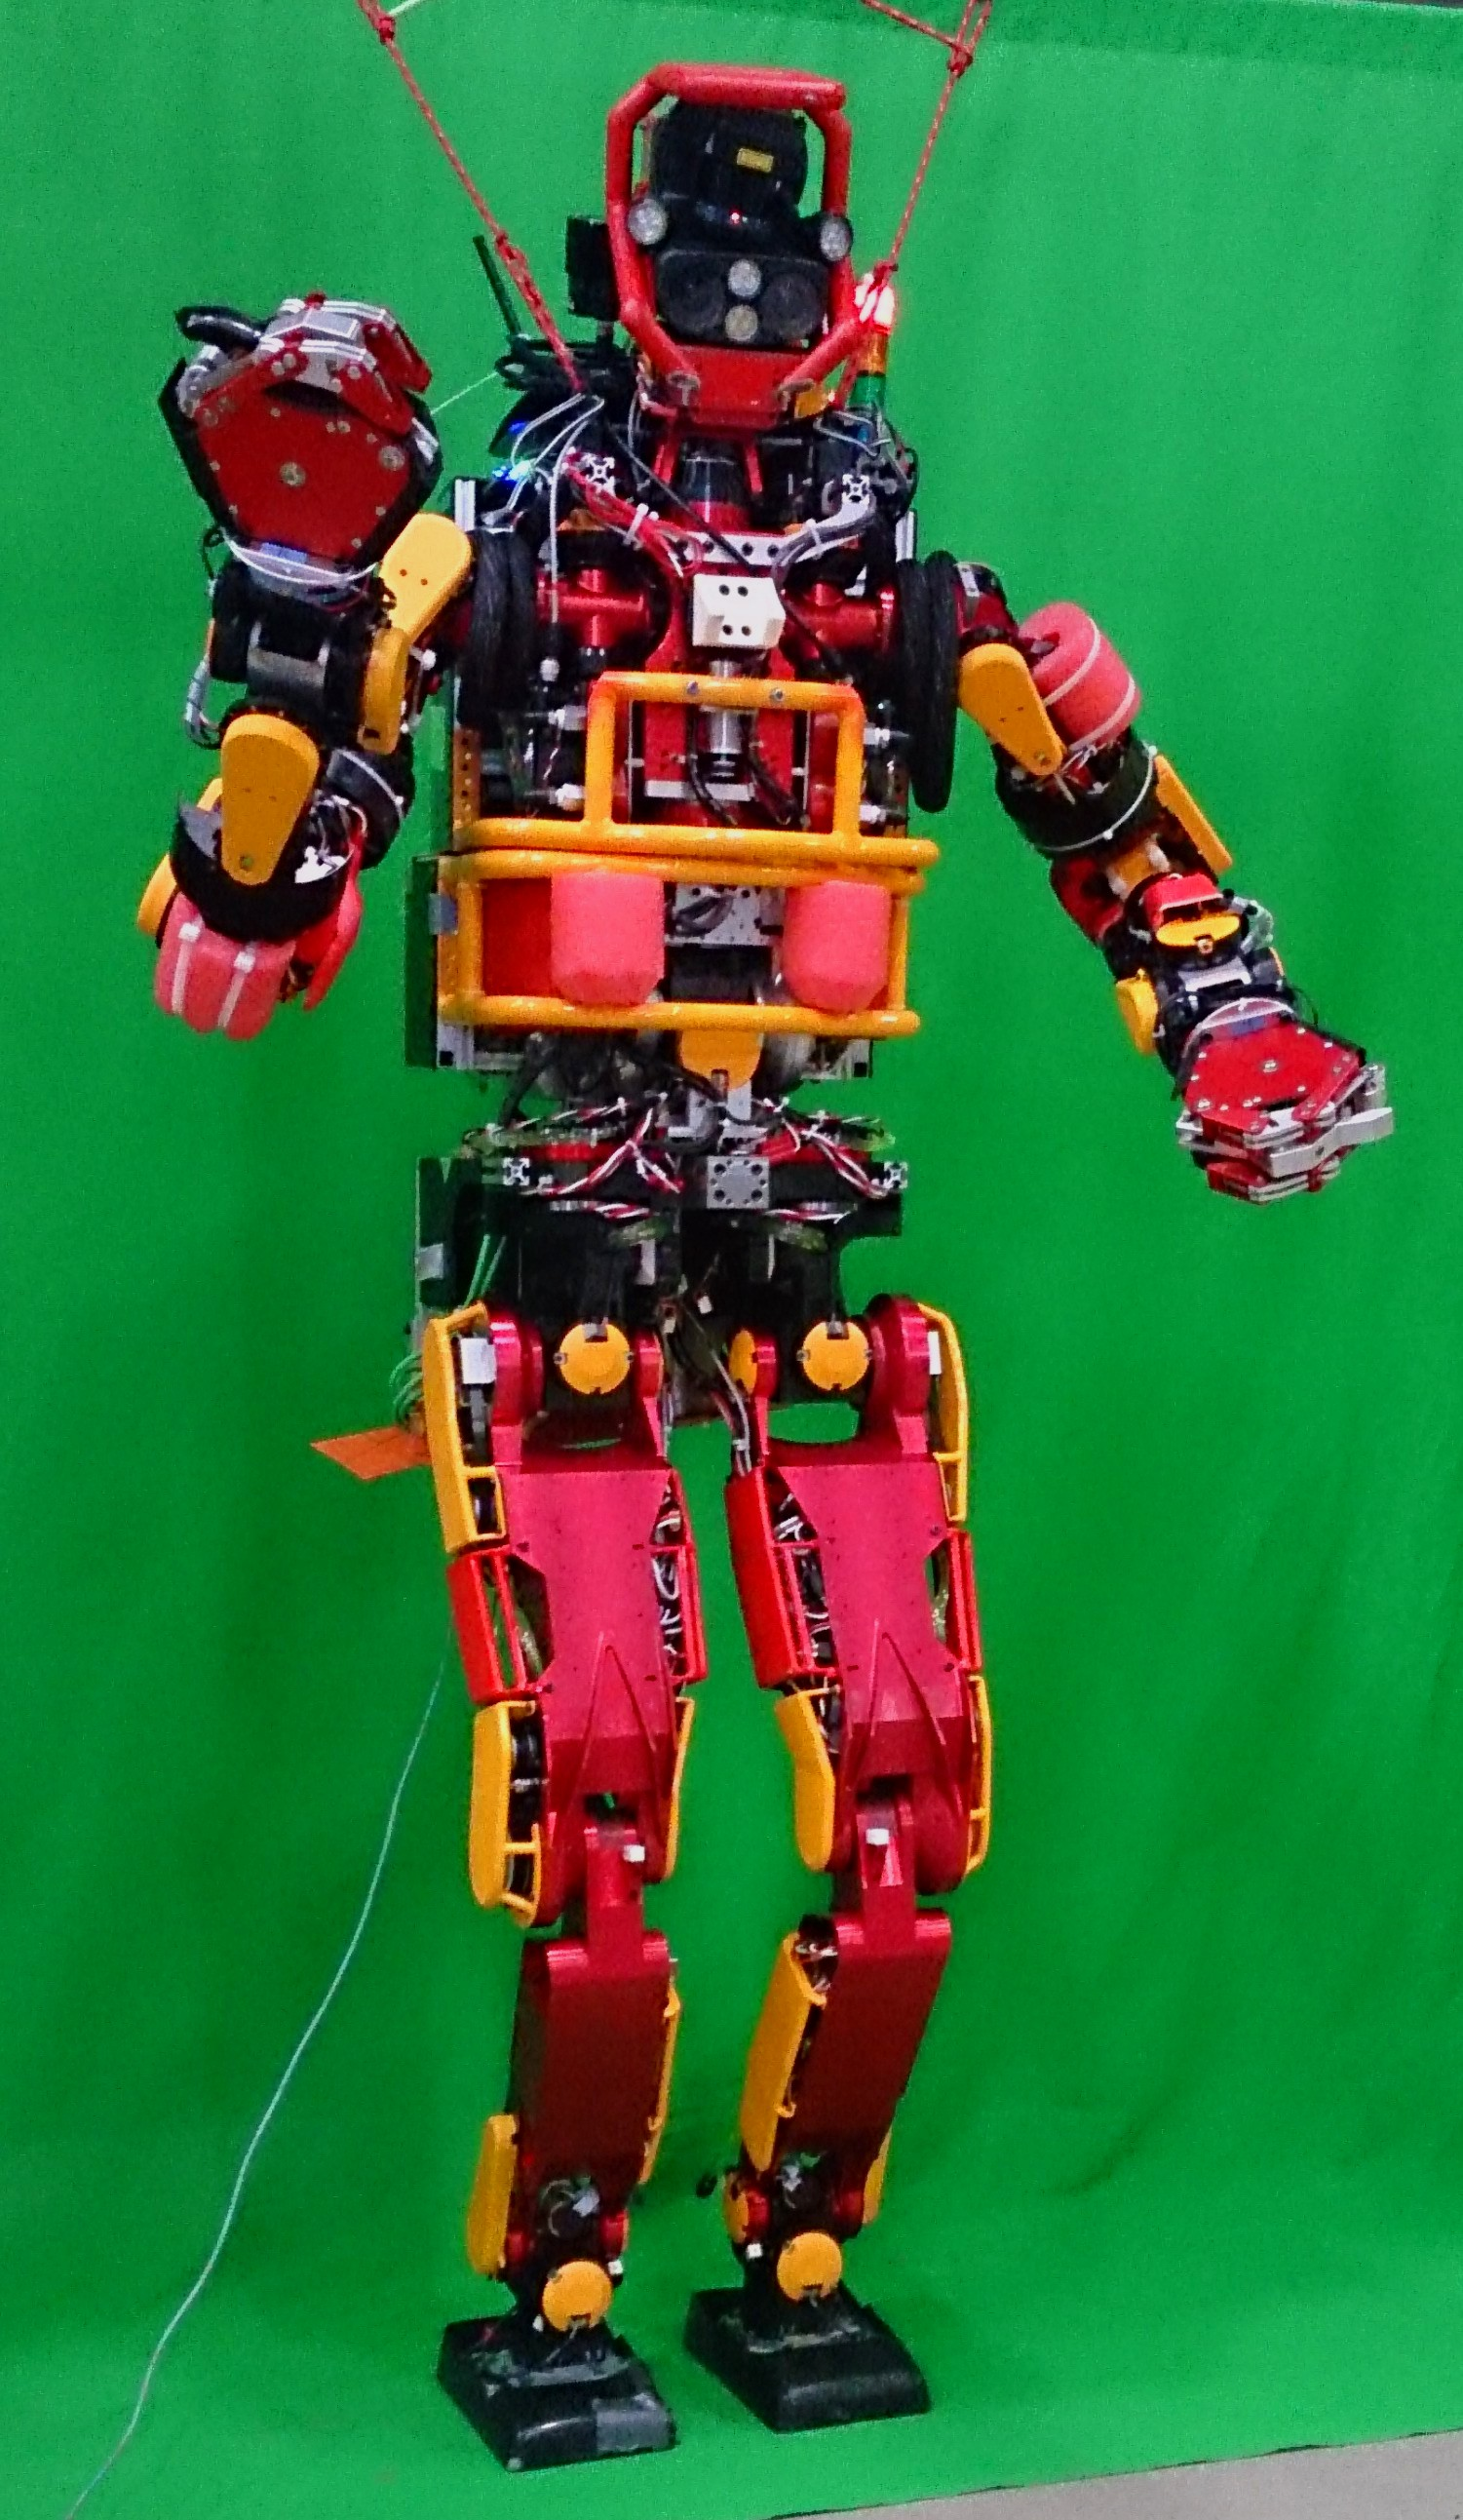
\includegraphics[width=\columnwidth]{jaxon2_appearance.png}
   \caption{JAXON2}
   \label{figure:est_graph}
  \end{minipage}
 \end{center}
\end{figure}




\section{検証実験}
認識、軌道予測、動作生成の評価をするための実験を行った
\subsection{実際のボール投球による認識と軌道予測実験}
ボールの三次元座標がどの程度のノイズを含んだ不確実な情報になっているかを確かめるため、実際にボールを投げ、各時刻のボールの三次元座標を計算すると共に、線形回帰によりどの程度正確に軌道予測が行えるのかを調べた。
動作生成を含まないため、カメラはロボットに搭載せずに実験を行った。

\figref{coords_graph}はボールの三次元座標の時間変化をプロットしたものであるが、どれも細かく振動しており、特に奥行き方向の座標がうまく取れていないことがわかる。\figref{est_graph}は\figref{coords_graph}の時間変化から計算したカメラから1m先の奥行き方向に対して垂直な平面上のどの座標にボールが来るかを予測したものであるが、全く予測できていないことがわかる。

\begin{figure}[tbh]
 \begin{center}
  \begin{minipage}{0.45\columnwidth}
   \includegraphics[width=\columnwidth]{coordinates_graph_316.png}
   \caption{座標の時間変化}
   \label{figure:coords_graph}
  \end{minipage}
  \hspace{0.05\columnwidth}
  \begin{minipage}{0.45\columnwidth}
   \includegraphics[width=\columnwidth]{coordinates_graph_316.png}
   \caption{軌道予測の時間変化}
   \label{figure:est_graph}
  \end{minipage}
 \end{center}
\end{figure}

二次元画像上での位置はよく認識できているが三次元座標を計算しようとすると奥行き方向がガタガタになる
動的な動きをするとカメラの非同期により同時刻に
\subsection{ボール位置にラケットを差し出す動作生成実験}
静的な物体の位置認識(x,y座標)は良く出来ていた
連続してikを解いていたため腕がねじれていくなどの問題があった

\section{今後の方針}
いろいろやってみたけど軌道予測もうまくいかないし、ikを解くのにも時間がかかるし完全に予測して理想の動きをしてしかも時間内に動作を行うのは無理
あらかじめ高速な複数の動作を準備しておいて、どれを呼び出すのかをできるだけ早く決める(逐次更新は難しい)
\subsection{学習手法について}
入力は初めのボールの座標を数点(これも正確とは限らない)、出力はどの動作を選びどのタイミングで再生するか
三次元座標の時系列座標を入力、
RNNなどを


\begin{table}[tbh]
 \begin{center}
  \begin{tabular}{|l|r|} \hline
  A1 & B1 \\
  A2 & B2 \\ \hline
  \end{tabular}
  \caption{図の参考例}
  \label{table:sample}
 \end{center}
\end{table}

\section{おわりに}

\bibliographystyle{junsrt}
\bibliography{p-report}


\end{document}

